\documentclass[12pt,letterpaper,fleqn]{article}

%       amslatex provides nice math extensions for typesetting mathematics
\usepackage{amsmath}
\usepackage{amsfonts}
\usepackage{tmmaths}
\usepackage{sympytex}

%       pstricks provides powerful environments for incorporating postscript into a
%       TeX/LaTeX document. You must have a postscript printer and a package like
%       dvips to convert the DVI file to a PS file.
%\usepackage{pst-all}
%\usepackage{pstricks,pst-plot}
%\usepackage{pst-coil,pst-node}

%  This package provides native tex support for numbered grids. The syntax is:
%  \graphpaper[spc](x_lowleft,y_lowleft)(x_upperright,y_upperright)

%\usepackage{graphpap}
%\usepackage{float}

%  The package below must be initialized with "\initfloatingfigs" immediately after the
%  "\begin{document} command.
%\usepackage{floatfig}

\usepackage{graphicx}
\graphicspath{{i:/mytex/graphics}}
\DeclareGraphicsExtensions{.ps,.eps}

%       tst is a package for the creation of exams, quizzes and tests. the include
%       file mathstuf (see below) provides many abbreviations for these environments.
%\usepackage{tst}

%       epsfig is a package which provides for the inclusion of Encapsulated PostScript
%       files in a document.
%\usepackage{epsfig}
%\usepackage{epic,eepic}
\include{mathstuf}
\usepackage[total={7.25in,10in},top=0.25in,left=0.75in,includehead]{geometry}
\usepackage{fancyhdr}
\pagestyle{fancy}
\lhead{Math 252}
\rhead{\large Name\makebox[2in]{\hrulefill}}
\chead{\LARGE Assignment 2}
%\lfoot{\today}
\cfoot{}
%\rfoot{\thepage}
\renewcommand{\headrulewidth}{0.4pt}
\renewcommand{\footrulewidth}{0.4pt}
\setlength{\parindent}{0pt}
\setlength{\parskip}{2ex}

\newcounter{tf}[enumi]
\newenvironment{tf}[0]{\begin{list}%
{\alph{tf}. \makebox[5em]{True\hfill False}}%
{\usecounter{tf}\setlength{\labelwidth}{7em}%
\setlength{\leftmargin}{3.5cm}%
\setlength{\labelsep}{1cm}}}%
{\end{list}}

%\usepackage{epic,eepic}
\newcommand{\numline}{%
%\newcounter{mark}%
%\setcounter{mark}{-1}%
\setlength{\unitlength}{0.1in}%
\begin{picture}(0,0)%
\thicklines%
\put(0,0){\line(1,0){60}}%
\multiput(0,0)(10,0){7}{\line(0,-1){1}%
\makebox(0,-1.5)[t]{\arabic{mark}}\stepcounter{mark}}%
%
\thinlines%
\multiput(0,0)(5,0){12}{\line(0,-1){0.5}}%
\multiput(0,0)(1,0){60}{\line(0,-1){0.3}}%
%\put(-5,265){\makebox(0,0)[l]{{\bf cm}}}%
\end{picture}}%

\newcommand{\ds}{\displaystyle}
\usepackage{amsfonts}


\let\oldhat\hat
\renewcommand{\hat}[1]{\oldhat{\boldsymbol{\mathbf{#1}}}}
\newcommand{\lv}[1]{\ensuremath{\langle #1 \rangle}}
\renewcommand{\i}{\ensuremath{\hat{\imath}}}
\renewcommand{\j}{\ensuremath{\hat{\jmath}}}
\renewcommand{\k}{\ensuremath{\mathbf{\oldhat{k}}}}
\newcommand{\ora}[1]{\ensuremath{\overrightarrow{#1}}}
\renewcommand{\vec}[1]{\ensuremath{\mathbf{#1}}}
\renewcommand{\v}[1]{\ensuremath{\vec{#1}}}
\newcommand{\abs}[1]{\ensuremath{\lvert #1 \rvert}}

\usepackage{tabularx}
\usepackage{paralist}
\newcommand{\red}[1]{\textcolor{red}{#1}}
\newcommand{\blue}[1]{\textcolor{blue}{#1}}
% \newcommand{\ans}[1]{\quad\fbox{answer: \red{#1}}}
\newcommand{\ans}[1]{\mbox{{\bf Ans:} \blue{#1}}}
\newcommand{\dd}[2][]{\ensuremath{\frac{\text{d}#1}{\text{d}#2}}}
\newcommand{\eval}[2]{\ensuremath{\left.#1\right|_{#2}}}

\usepackage{wrapfig}

\begin{document}
\section*{Simpson's Rule}
Simpson's rule is a formula which allows us to approximate the value of a definite integral for those situations when it is either difficult or impossible to ust the Fundamental Theorem of Calculus. To approximate the value of the definite integral
\begin{equation*}
	\int_a^b f(x)\;dx
\end{equation*}
we partition the interval $[a, b]$ into an \emph{even} number $n$ of subintervals of equal width $\Delta x$ with partition points $a=x_0, x_1,\ldots,x_n=b$. Simpson's rule tells us that
\begin{equation*}
	\int_a^b f(x)\;dx \approx \frac{1}{3}\Delta x\left(f(x_0) + 4f(x_1) + 2f(x_2) + \cdots + 4f(x_{n-2}) + 2f(x_{n-1}) + f(x_n)\right)
\end{equation*}
where the error $E_S$ (the difference between the exact value of the integral and the approximation) can be estimated by
\begin{equation*}
	|E_S| \leq \frac{K (b-a)^5}{180n^4}
\end{equation*}
with $K$ a constant such that $\left|f^{(4)}(x)\right| \leq K$, $\forall x\in [a,b]$.
\subsection*{Problems}
\begin{enumerate}
  \item A sky diver jumps out of a plane at time $t=0$ seconds, opens his parachute two minutes later and lands five minutes after his jump. The table below shows his speed $v(t)$ (in meters per second) at different times $t$ (in seconds) during his jump. The distance he fell is given by the integral $\int_0^{300} v(t)\;dt$. Use Simpson's rule to estimate this distance.
  \begin{table}[htbp]
    \centering
    \begin{tabularx}{0.8\textwidth}{| l | X | X | X | X | X | X | X | X | X | X | X | X | X| }
        \hline
        $t$ & 0 & 25 & 50 & 75 & 100 & 125 & 150 & 175 & 200 & 225 & 250 & 275 & 300\\ \hline
        $v(t)$ & 0 & 176 & 264 & 307 & 329 & 294 & 159 & 100 & 74 & 63 & 59 & 57 & 56\\ \hline
    \end{tabularx}
\end{table}
\newpage
    \item Let $f(x) = \sin(x^2)$.
	\begin{enumerate}
		\item Use Simpson's rule with $n = 8$ subintervals to approximate the value of $\int_0^\pi f(x)\;dx$.
		\item Use the error estimation formula for Simpson's rule to estimate the error between the exact value of the integral and the approximation. Use the graph of the fourth derivative of $f$ below, to determine a value for $K$ in the formula that gives the best error bound.
	\end{enumerate}
\begin{figure}[!htb]
	\centering
	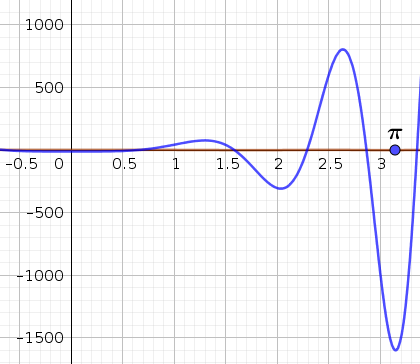
\includegraphics[width=0.4\textwidth]{img/FourthDerivOfSin_x2.png}
	\caption{Graph of $f^{(4)}(x)$}
	\label{}
\end{figure}
\end{enumerate}
\end{document}
